\chapter{Topological band theory}
\label{ch:topo-intro}
In this chapter, we introduce more formally the concept of topology in the band theory. We provide the definitions of topological invariants, precise the bulk-boundary correspondence, and discuss the details of the classification for gapped free-fermion models.


\section{Notion of topology}
Topology is a branch of mathematics that deals with properties of smooth, continuous transformations. It ignores the geometrical details of an object, but rather focuses on global features that can be described by topological invariants We briefly introduce fundamental concepts~\cite{Nakahara}.

\begin{figure}[H]
\centering
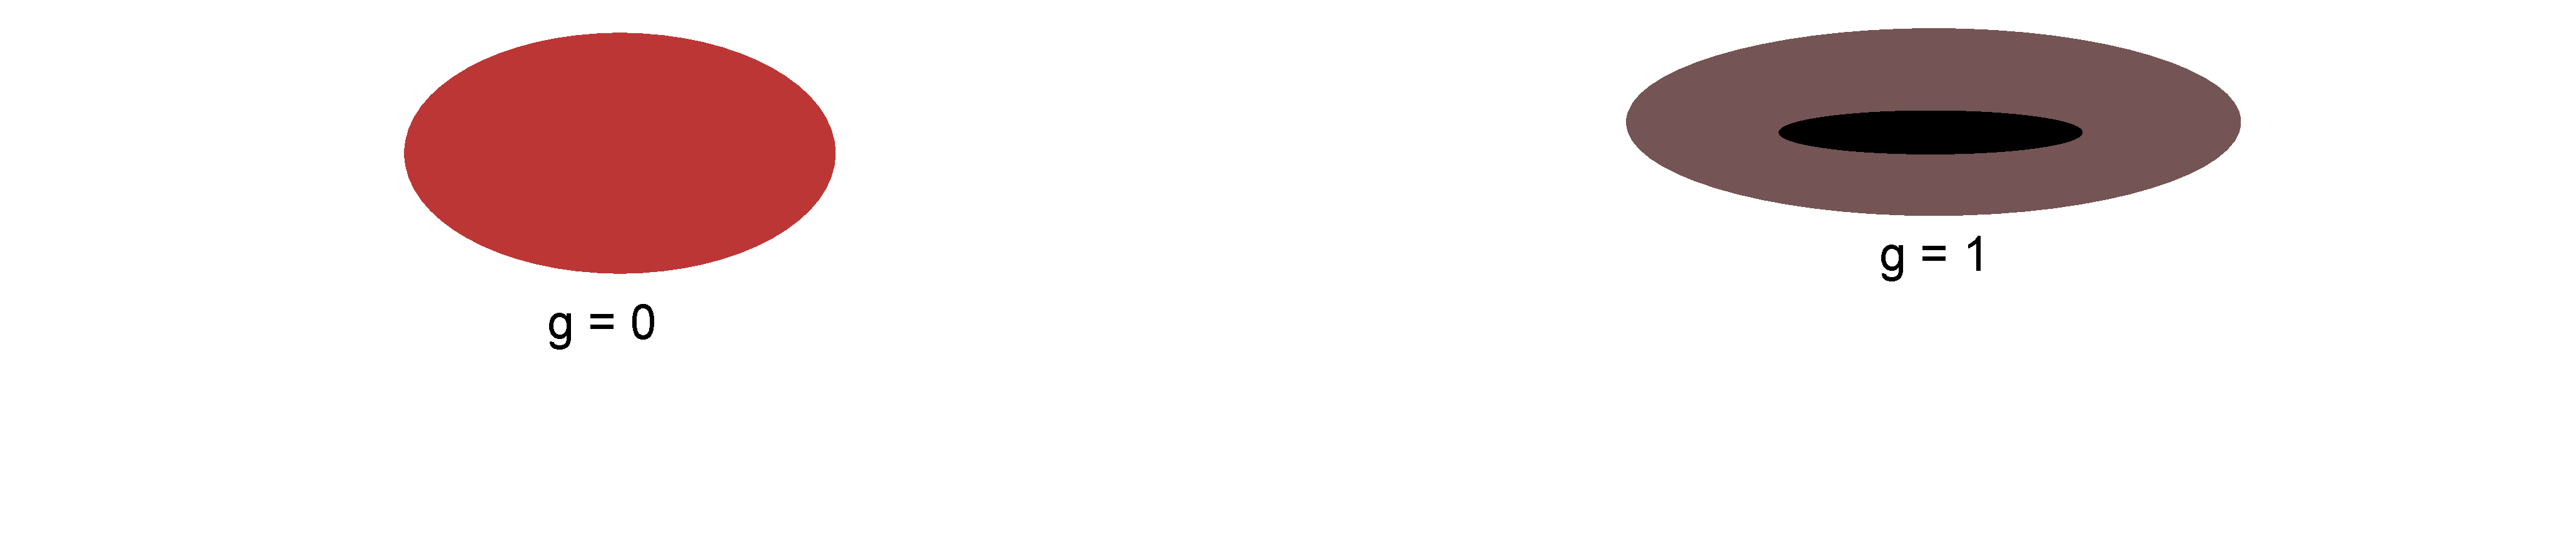
\includegraphics[width = 0.8\textwidth]{intro_genus.pdf}
\caption{From a perspective of topology, the}
\end{figure}

\subsection{Homotopy and equivalence classes}
Consider two smooth manifolds $X, Y$. Then continuous maps $f_0 : X \rightarrow Y$ and $f_0 : X \right Y$ are homotopically equivalent if there is a continuous maps
\begin{equation}
F : [0, 1] \times X \rightarrow Y
\end{equation}
$F(0,x) = f_0 (x)$ and $F(1,x) = f_1 (x)$ for all $x \in X$.


Hence, in order to change

%\subsection{Topological equivalence}
%Topology cares about the smooth, continuous deformations
%
%
%
%If the system has a translational invariance, then the states can be represented in the form of Bloch states labeled by the band index $n$ and momenta $k$.
%
%
%\subsection{Bulk-boundary correspondence}
%There's another striking consequence of non-trivial (non-zero) bulk topological index - the presence of protected gapless edge modes in the open geometry. Even though there's no rigorous proof for the bulk-boundary correspondence, it works remarkably well.


\section{Symmetries and classification of topological insulators and superconductors}



In quantum mechanics, the symmetries are constructed according to the Wigner's theorem: they are the operators that preserve transition probabilities and are therefore implemented via unitaries or antiunitaries which commute with the Hamiltonian. 

A local unitary symmetry can be decomposed as $U = U_1 \ldots U_n$, where each $U_i$ affects only a small region in space. Conversely, a non-local unitary 

A fundamental example of antiunitary operator is the time-reversal, which takes $t \rightarrow -t$. Acting on Hamiltonian $H$:
\begin{equation}
\mathcal{T}  H \mathcal{T}^{-1} = + H
\end{equation}
As all antiunitary operators, $\mathcal{T}$ can be decomposed into a product of a unitary operator $T$ and complex conjugate $\mathcal{K}$, $\mathcal{T} = T \mathcal{K}$. Applying $\mathcal{T}$ twice will lead to the rise of the phase factor, hence $\mathcal{T}^2 = \pm 1$. This is true for all antiunitary symmetries. For spin-1/2 systems, TRS systems follow the Kramers' theorem which tells that all states comes in time-reversal symmetric pairs $\mathcal{T} \ket{n} = \ket{n}$.

Another (antiunitary) symmetry is the particle-hole $\mathcal{P}$, defined as:
\begin{equation}
\mathcal{P}  H \mathcal{P}^{-1} = - H
\end{equation}

Finally, we can define chiral symmetry being a product of $\mathcal{T}$ and $\mathcal{P}$, $\mathcal{C}= \mathcal{TP}$ \footnote{Note that $\mathcal{P}$ and $\mathcal{C}$ anticommute with the single-particle Hamiltonian}
\begin{equation}
\mathcal{C}  H \mathcal{C}^{-1} = - H
\end{equation}
$\mathcal{C}$ may be present in the system, even if $\mathcal{T}$ and $\mathcal{P}$ are absent. Although chiral symmetry in not a symmetry in a strict sense, but guarantees that non-zero eigenvalues of the Hamiltonian come in pairs, hence there is a spectral symmetry.




Dates back to the idea of \'{E}lie Cartan's classification of symmetric spaces in differential geometry. Later on, Altland and Zirnbauer applied this classification in the context of random matrix theory~\cite{AltlandZirnbauer1997}




\begin{table}
\centering
\begin{tabular}{|c|c||c|c|c||c|c|c|c|}
\hline
 & & $\mathcal{T}$ & $\mathcal{P}$ & $\mathcal{C}$ & 1 & 2 & 3 & 4 & 5 & 6 & 7 & 8 \\
\hline
\hline
standard & A (unitary) & 0 & 0 & 0 & - & $\mathbb{Z}$ & - &   $\mathbb{Z}$ & - &  $\mathbb{Z}$  & -  $\mathbb{Z}$ \\ 
\cline{2-8}
 & AI (orthogonal) & +1 & 0 & 0 & - & - & - \\
\cline{2-8}
 & AII (symplectic) & -1 & 0 & 0 & - & $\mathbb{Z}_2$ & $\mathbb{Z}_2$ \\
\hline
\hline
 chiral & AIII (chiral unitary) & 0 & 0 & 1 & $\mathbb{Z}$ & - & $\mathbb{Z}$ & - & $\mathbb{Z}$ & - & $\mathbb{Z}$  & -\\
\cline{2-8}
 & BDI (chiral orthogonal) & +1 & +1 & 1 & $\mathbb{Z}$ & - & - \\
\cline{2-8}
 & CII (chiral symplectic) & -1 & -1 & 1 & $\mathbb{Z}$ & - & $\mathbb{Z}_2$ \\
\hline
\hline
BdG & D & 0 & +1 & 0 & $\mathbb{Z}_2$ & $\mathbb{Z}$ & - \\
\cline{2-8}
& C & 0 & -1 & 0 & - & $\mathbb{Z}$ & - \\
\cline{2-8}
 & DIII & -1 & +1 & 1 &  $\mathbb{Z}_2$ &  $\mathbb{Z}_2$ &  $\mathbb{Z}$ \\
\cline{2-8}
 & CI & +1 & -1 & 1 & - & - & $\mathbb{Z}$ \\
\hline
\end{tabular}
\caption{Table of symmetry classes of non-interacting Hamiltonians. 0 corresponds to the absence of symmetry and $\pm$ 1 indicates the sign to which the symmetry squares

}
\label{tab:10fold}
\end{table}

All possible combination of internal symmetries in $d = 1, \ldots, 8$ spatial dimensions are tabulated in Tab.~\ref{tab:10fold}. There are ten distinguished classes.

This was first proposed in Ref.~\cite{10foldSchnyder2008}, with further mathematical improvements from K-theory (such is pattern called Bott periodicity; with a period two for the complex classes AI, AIII and a period eight for remaining eight real classes) given by Kitavev~\cite{10foldKitaev2009} to finally provide the complete classification \cite{10foldRyu2010}.

For higher dimensions, topological invariants repeat themselves and show the Bott periodicity with period 2 for classes A and AIII, and period 8 for the remaining ones.

\section{Topological invariants}
\subsection{Geometrical phases and adiabatic evolution}



Berry connection of Bloch states:
\begin{equation}
\mathbf{A} = i \braket{u_n (\mathbf{k} )| \Delta  | u_m (\mathbf{k} ) }
\label{eq:berryconn}
\end{equation}

$\Delta \equiv  \Delta_{\mathbf{k}$
Berry curvature: 
\begin{equation}
F = \Delta \times \textbf{A}
\label{eq:berrycurv}
\end{equation}



Gauss-Bonnet theorem for a two-dimensional manifold $M$ without a boundary:
\begin{equation}
\int_M K dA = 2 \pi (2 - 2g)
\label{eq:gaussbonnet}
\end{equation}
with $K$ being the Gauss curvature and $g$ - genus.

\subsection{Chern number}

For two-dimensions, it is given by the (first) Chern number:
\begin{equation}
C = \frac{1}{2 \pi} \int_{BZ} F
\label{eq:chern}
\end{equation}
(note, some conventions incorporate imaginary unit $i$ explicitly in the prefactor).

\subsection{$Z_2$ topological index}


Some systems can have one trivial and one topological phase, which is characterized by a two-valued index $\nu$ being 0 or 1, respectively. $Z_2$ invariant can be computed easily in the presence of inversion symmetry using Fu-Kane formula~\cite{FuKane2007}:
\begin{equation}
\delta_i = \prod_{m = 1}^N  \xi_{2m} (\Gamma_i); \hspace*{2cm} (-1)^{\nu} = \prod_i \delta_i
\label{eq:fukane}
\end{equation}
where $\Gamma_i$ are time-reversal invariant momenta in the BZ, $\xi_{2m} (\Gamma_i)$ is every second occupied Kramers pair. In case of 3D systems, two types of TI can be observed, defined whether they have a strong or weak indices. Non-zero strong index means that the system cannot be seen as a set of stacked 2D layers, it's intrinsically three-dimensional.

Because for TRS systems $C$ always vanishes, if $S_z$ (spin component pointing out of 2D plane) is conserved, one may define the spin Chern number~\cite{ShengCs2006} based on the fact that spins up and down have independent Chern numbers:
\begin{equation}
C_s = \frac{C_{\uparrow} - C_{\downarrow}}{2}
\label{eq:spinchern}
\end{equation}
and is related to $\nu$ as $\nu = C_s \mod 2$



Pffafian formalism 

\section{Topical examples}
In the following, we would like to discuss relevant examples of toy models and discuss experimental realizations.

\subsection{Class BDI: Su-Schriffer-Heeger chain}
SSH model, firstly proposed to describe polyacetylene, describes spinless fermions in 1D chain~\cite{SSH1976}

\begin{figure}[H]
\centering
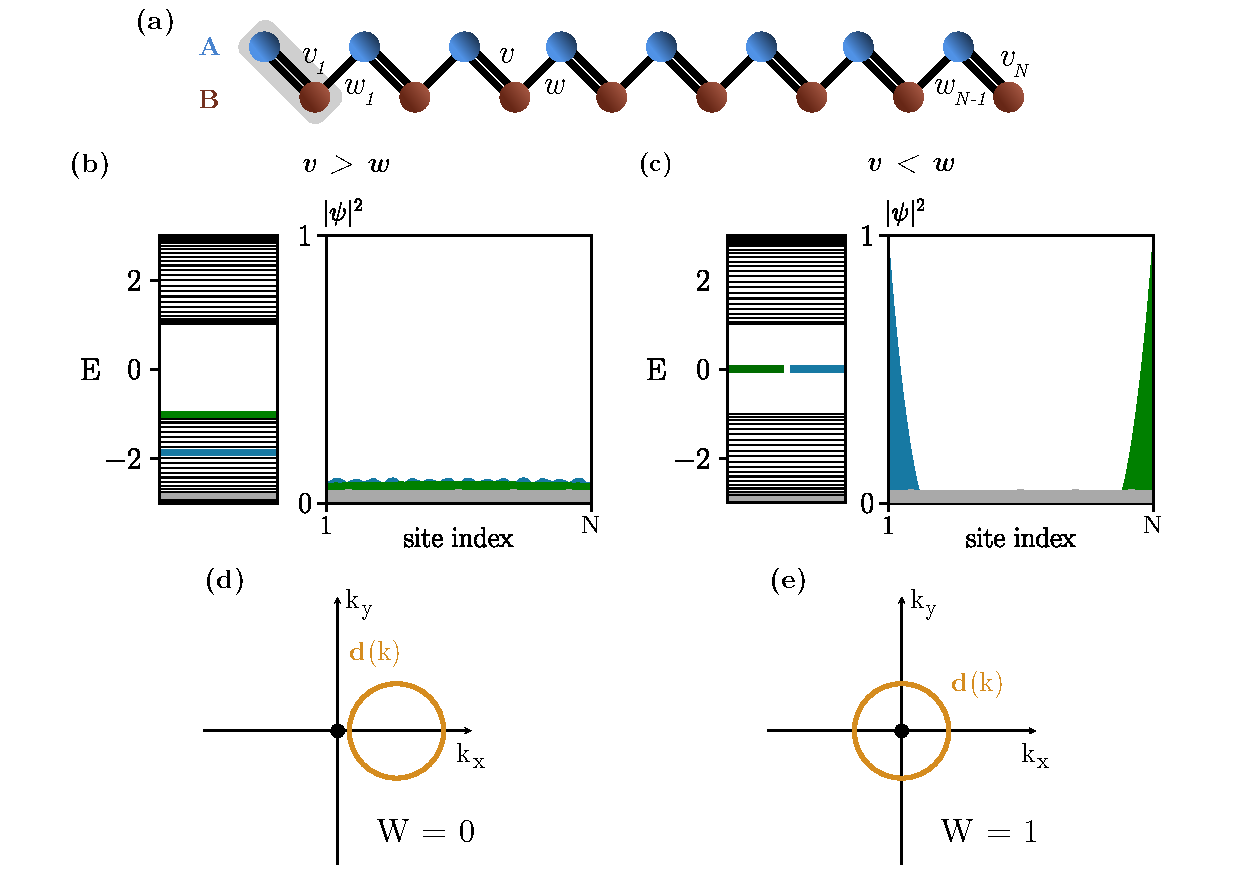
\includegraphics[width=\columnwidth]{intro_ssh.pdf}
\caption{A schematic of SSH chain. There are two atomic sites $A$ and $B$ per unit cell and alternating hoppings with strength $t$ (within unit cell) and $t'$ (between neighbouring unit cells). Depending on $t$ and $t'$,  the model exhibits two phases: if $t' > t$, the system is in a topological phase with gapless edge modes in an open geometry; conversely, if $t' < t$ the system is in a trivial phase with $t' = 0$ as a fully dimerized case.}
\label{fig:ssh}
\end{figure}

Bloch Hamiltonian reads:
\begin{equation}
H (k) = \begin{pmatrix}
0 & t + t' e^{i k} \\
t + t' e^{-i k} & 0
\end{pmatrix}
\label{eq:ssh}
\end{equation}
Dispersion
\begin{equation}
E(k) = \pm \sqrt{t^2 + t'^2 + 2 t t' \cos k}
\end{equation}



The system has the chiral symmetry realized by $\sigma_z$, particle-hole $P = \sigma_z \mathcal{K}$ and time-reversal $\mathcal{T} = \mathcal{K}$. Here, It is the chiral symmetry that protects the topological properties and, for instance, adding long range hoppings would destroy topological states.


\subsection{Class A}
\subsubsection{Quantum Hall effect}
IQH states can be seen as the most robust topological states without intrinsic topological order as they don't need any symmetry to persist. In particular, TR is broken. Actually, in the classification based on the entanglement (Wen vs. Kitaev),


Let us start from a semiclassical description of the QH effect. In the bulk, electrons do not move freely through the sample, but rather follow circular trajectories with a radius $l_B = \sqrt{\hbar / eB}$. However, at the edges the orbits do not form closed loops and contribute to the current flow. Edge current will not disappear in presence of disorder and is not affected by the detailed shape of a sample. Recall the 





A consequence of non-trivial bulk topology is the presence of gapless edge modes at the interface between systems with different topologies (for instance, trivial vacuum). They are chiral, that is, they propagate along the edge only in one direction.

\subsubsection{Chern insulators}
Haldane model is a canonical example of a Chern insulator. It describes spinless electrons in a single honeycomb lattice, where staggered potential $M$ breaks inversion symmetry and the complex next-nearest-neighbour hoppings breaking TR symmetry arise due to to Aharanov-Bohm phases. It is possible to choose the AB phases such that net magnetic field in an unit cell is zero (in contrast to the quantum Hall effect).




Peierls substitution:
\begin{equation}
r_{xy} \rightarrow t_{xy} \exp \left( -\textnormal{i} \frac{e}{h} \int_{\Gamma} \mathbf{A} \cdot d \ell \right)
\label{eq:peierls}
\end{equation}
Staggered mass term $M$ is defined 



\begin{equation}
H_{Haldane} = -t \sum_{\langle i, j \rangle} \hat{c}^{\dagger}_i \hat{c}_j - t' \sum_{\langle \langle i, j \rangle \rangle} e^{\mathrm{i} \phi} \hat{c}^{\dagger}_i \hat{c}_j  + \sum_i M_i \hat{c}^{\dagger}_i \hat{c}_j  + h. c.,
\end{equation}
where $ \langle \ldots \rangle$ corresponds to real-valued hoppings between nearest neighbours, and $ \langle \langle \ldots \rangle \range$ to the next-nearest neighbours


Experimental realizations include fermionic ultracold atoms~\cite{Jotzu2014} or classical wave systems~\cite{CIacustic2019}.
\subsection{Class AII: quantum spin Hall effect}
In 2005, Kane and Mele extended the notion of Chern insulators by taking two copies of Haldane model with opposite chiralities~\cite{KaneMeleGraphene}. This lead to the construction of a insulating state which is time-reversal invariant and has protected gapless edge modes lying in the bulk gap, where the topological properties are defined by a $\mathbf{Z}_2$ invariant. Edge states are helical - that is, they two states counterpropagate along a boundary They also come in time-reversal pairs according to the Kramers' theorem. States with odd number of Kramers' edge pairs are topological, while with even number - are topologically trivial. Another consequence of the TR symmetry is that energy levels crossing appear only at special points in the BZ. Authors suggested that this model may be realized in graphene, however due to negligible spin-orbit coupling, it is not realizable experimentally under realistic conditions~\cite{PhysRevB.74.165310, PhysRevB.75.041401}. Besides fundamental theoretical interest, QSH states hold great promise for spintronics as it is possible to manipulate spin degrees of freedom in the absence of magnetic field~\cite{RevModPhys.82.3045}.

\begin{figure}
\centering
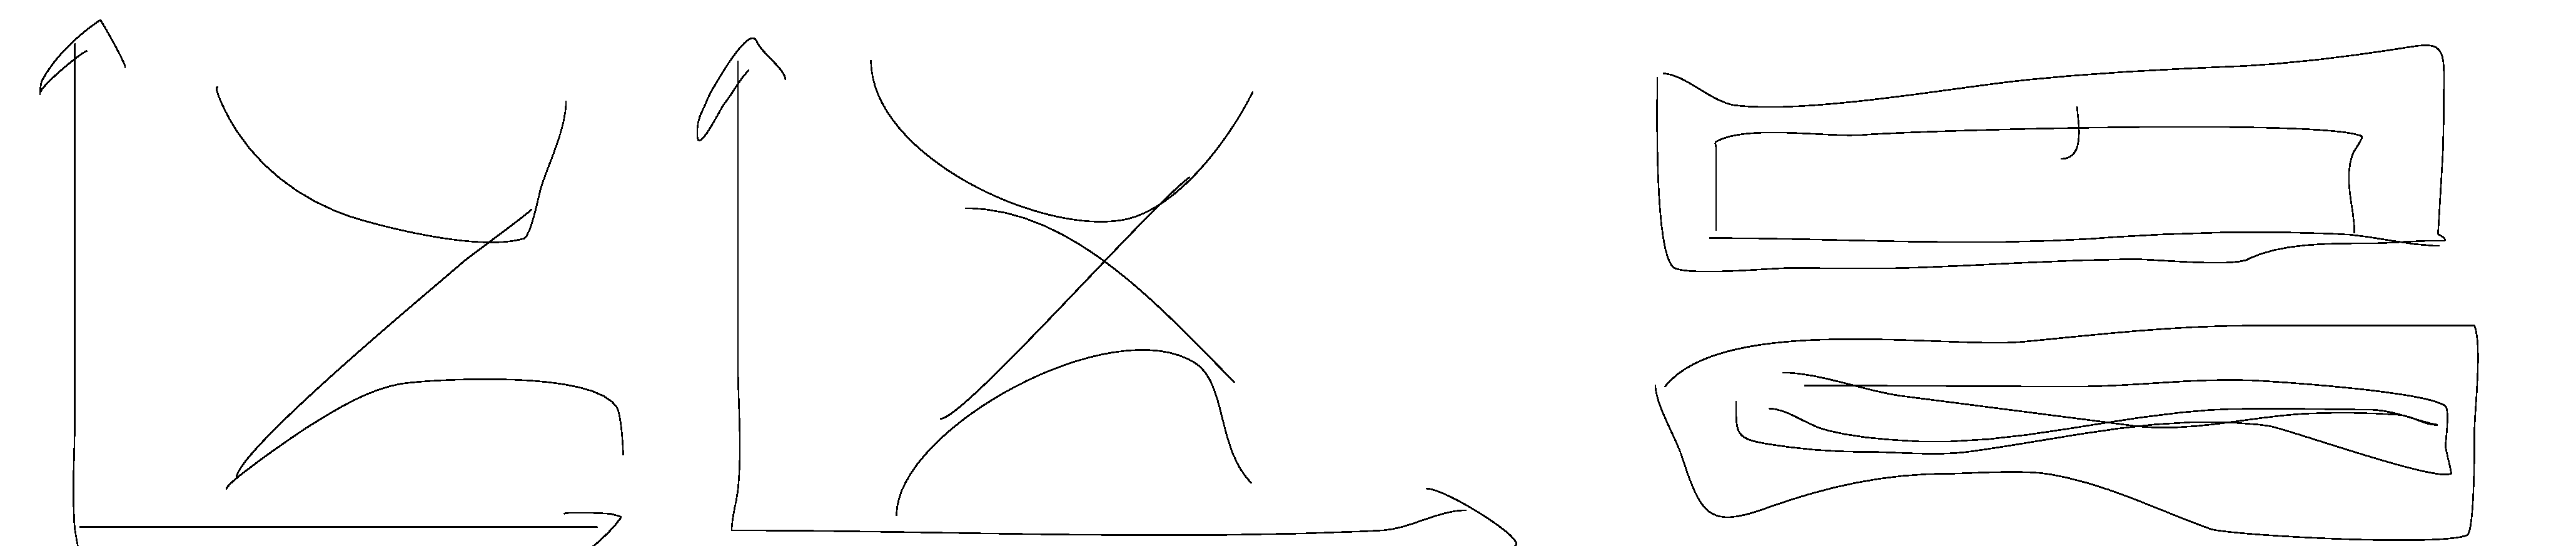
\includegraphics[width=\columnwidth]{intro_qheqshe.pdf}
\caption{Left: Schematic representation of the band structures of (a) Chern insulator with $C = +1$ and (b) QSH system constructed as two copies of CI with opposite Chern numbers, together with conserved z-spin component. Right: Edge modes flowing in samples}

\label{fig:qheqshe}
\end{figure}

Subsequently, QSH effect was proposed in strained zinc-blende semiconductors (such as gallium arsenide)~\cite{BernevigQSHE2006}. Bernevig, Hughes and Zhang~\cite{Bernevig1757} predicted a quantum phase transition in HgTe/CdTe quantum wells as a function of the thickness. This happens because of a band inversion due to strong spin-orbit coupling in HgTe: CB has a $p$-like character and  VB is composed of $s$-orbitals instead of normal ordering which is observed in CdTe: $s$-orbital character of conduction band and $p$-orbital of valence band. It was confirmed experimentally year later by observing quantized resistance $h^2 / 2e$ (factor 2 comes from the spin contribution) ~\cite{MolenkampQSHE2007}. This ignited a search for new materials exhibiting QSH states~\cite{PhysRevLett.100.236601,PhysRevLett.107.136603}, and topological insulators in three-dimensions.





In Ref.~\cite{MurakamiBi2006}

\clearpage